\label{app:long_motion}

In this section we shall define some key parameters of longitudinal motion to aid understanding of the effects of wakefields on particle beams. This text follows closely the introductions to longitudinal motion given by Métral \cite{Metral:LongDyn} and Le Duff \cite{Leduff:LongDyn}. A significant parameter in the case longitudinal dynamics and RF control is the parameter known as the momentum compaction factor. This is defined relating the variation in the closed orbit with momentum. For example, if we consider a nominal closed orbit in a circular accelerator of length $C$, defined for a particle of momentum $p$. For a particle with a momentum deviation $\Delta p$ which gives a orbit length variation $\Delta C$, they are related to one another by

\begin{equation}
\frac{\Delta C}{C} = \alpha_{p} \frac{\Delta p}{p}
\end{equation}

assuming that the bending field $B$ is constant. In this case $C=2\pi R$ where $R$ is the average radius of the closed orbit. This maybe related by infinitessimal changes to give

\begin{equation}
\alpha_{p} = \frac{\frac{dC}{C}}{\frac{dp}{p}} = \frac{\frac{dR}{R}}{\frac{dp}{p}}
\label{eqn:momCP}
\end{equation}

and related to the dispersion of the optics and the bending radius $\rho$

\begin{equation}
\alpha_{p} = \frac{1}{C}\int_{C}\frac{D_{x} \left( s \right)}{\rho\left( s \right)} ds.
\end{equation}

For most circular machines $\alpha_{p}$ is positive, i.e. higher momentum means longer circumference of the orbit. To relate the momentum compaction to the particle energy, it can be seen that 

\begin{equation}
E = \frac{pc}{\beta} \rightarrow \frac{dE}{E} = \beta^{2}\frac{dp}{p}
\end{equation}

which substituting into Eqn.~\ref{eqn:momCP} gives

\begin{equation}
\alpha_{p} = \beta^{2}\frac{E}{R}\frac{dR}{dE}.
\end{equation}

For a machine with a positive momentum compaction, there are two relationships:

\begin{enumerate}
\item{a momentum larger than nominal results in an increased circumference of the orbit}
\item{a momentum larger than nominal results in an increase in velocity}
\end{enumerate}

If we consider what happens to the revolution frequency, we can see that at low energies, the velocity increases faster than C. At high energies, $v \approx c$ and remains almost constant, thus increases slower than C. There is an energy for which the velocity increase is compensated for by the increase in circumference, i.e. the revolution frequency doesn't change with increasing momentum. This is called the transition energy. Below this energy (below transition) increasing the energy of the particles results in a higher revolution frequency. Above the energy (above transition) increasing the energy of the particles results in a lower revolution frequency.

An additional useful factor to define is the slip factor $\eta$, defined as the revolution frequency spread per unit of momentum spread

\begin{equation}
\eta = \frac{\frac{df_{res}}{f_{res}}}{\frac{dp}{p}} = \frac{\frac{d\omega_{res}}{\omega_{res}}}{\frac{dp}{p}}.
\end{equation}

Considering that $f_{res} = v/C$, if follows that

\begin{equation}
\frac{df}{f} = \frac{d\beta}{\beta} - \frac{dC}{C}
\end{equation}

and similarly following from $p=\frac{mc\beta}{\sqrt{1-\beta^{2}}}$ is can be seen that

\begin{equation}
\frac{d\beta}{\beta} = \frac{1}{\gamma^{2}}\frac{dp}{p}
\end{equation}

which when considering Eqn.~\ref{eqn:momCP} leads to 

\begin{equation}
\frac{df_{res}}{f_{res}} = \left( \frac{1}{\gamma^{2}} -\alpha_{p}\right) \frac{dp}{p} = \eta \frac{dp}{p}.
\end{equation}

The transition energy is the energy for which $\eta=0$, given by the relativistic $\gamma$ factor at transition $\gamma_{tr}$

\begin{equation}
\gamma_{tr} = \sqrt{\frac{1}{\alpha_{p}}}.
\end{equation}

Thus 

\begin{equation}
\eta = \frac{1}{\gamma^{2}} - \frac{1}{\gamma_{tr}^{2}}.
\end{equation}

It's thus seen that for particles above transition $\eta < 0$ and below transition $\eta > 0$.

\section{Longitudinal Equations of Motion}

Here shall be given a brief overview of the longitudinal equations of motion of a non-synchronous particle in an RF bucket. The momentum offset and the particles phase can be given by

\begin{align}
\frac{d\left( \Delta p \right)}{dt} & =  A\left( sin \phi - sin \phi_{s} \right) \\
\frac{d\phi}{dt} & =  B \Delta p
\end{align}

where $A=(e\vec{V}_{rf})/(2\pi r_{s})$ and $B=-(\eta h)/(p_{s})(\beta_{s}c)/(r_{s})$ where $r$ is the particle orbit radius, $\vec{V}_{rf}$ is the peak RF voltage, $h$ is the RF harmonic and the subscript $s$ denotes the synchronous particle. Combining the above two equations we get to

\begin{equation}
\frac{d}{dt}\left( \frac{1}{B} \frac{d\phi}{dt} \right) - A \left( sin \phi - sin \phi_{s} \right) = 0
\label{eqn:GenLongMot}.
\end{equation}

If it is assumed that $A$ and $B$ change much more slowly than $\Delta \phi = \phi - \phi_{s}$, i.e. that significant acceleration occurs on a longer timescale than synchrotron oscillations, then this can be rewritten as

\begin{equation}
\frac{d^{2}\phi}{dt^{2}} + \frac{\Omega_{s}^{2}}{cos \phi_{s}} \left( sin\phi - sin\phi_{s} \right) = 0
\label{eqn:phiEOM}
\end{equation}

where 

\begin{equation}
\frac{\Omega_{s}^{2}}{cos\phi_{s}} = -AB = \Omega_{0}^{2} = \frac{e\vec{V}_{rf}\eta hc^{2}}{2\pi r_{s}^{2}E_{s}}.
\end{equation}

Subsequently we can make what is known as the small amplitude approximation, such that $\phi = \phi_{s} + \Delta \phi$. In this case it follows that

\begin{align}
sin \phi &= sin \left( \phi_{s} + \Delta \phi \right) \\
&= sin\phi_{s}cos\Delta \phi + cos\phi_{s} sin \Delta \phi \\
& \approx sin\phi_{s} + cos \phi_{s} \Delta \phi.
\end{align}

Similarly it can be seen that

\begin{equation}
\frac{d\phi}{dt} = 0 \Rightarrow \frac{d^{2}}{dt^{2}} = \frac{d^{2}}{dt^{2}}\left( \phi_{s} + \Delta \phi \right) = \frac{d^{2}\Delta \phi}{dt^{2}}
\end{equation}

which subsequently leads to small amplitude approximation of Eqn.~\ref{eqn:phiEOM}

\begin{equation}
\frac{d^{2}\Delta \phi}{dt^{2}} + \Omega_{s}^{2}\Delta \phi = 0.
\end{equation}

$\Omega_{s}$ s known as the synchrotron frequency, in this case of the harmonic oscillator represented by the non-synchronous particle. For accelerator stability is obtained when $\Omega_{s}^{2} > 0$. $\Omega_{s}^{2}$ is given by

\begin{equation}
\Omega_{s}^{2} = \frac{e\vec{V}_{rf}\eta hc^{2}}{2\pi r_{s} E_{s}} cos \phi_{s} \Rightarrow \Omega_{s}^{2} > 0 \Leftrightarrow \eta cos\phi_{s} > 0.
\end{equation}

This condition to an effect known as phase stability, wherein the stable phase of a particle relative to the RF phase is dependent on whether it is above or below transition. The stability of the particle oscillations relative to the RF phase are shown in Fig.~\ref{fig:longPhase}. It is interesting to note that when the particles cross the transition energy the stable phase changes drastically. In this case complex RF gymnastics are required to cross transition and remain stable.

\begin{figure}
\begin{center}
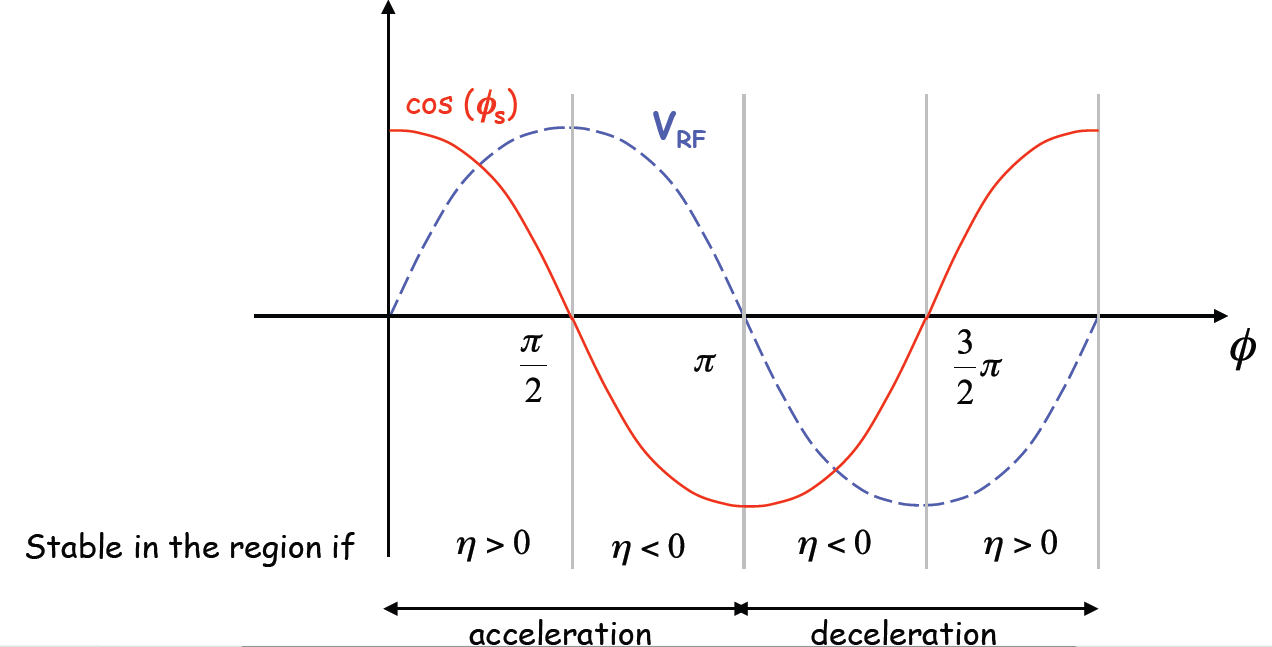
\includegraphics[width=0.75\textwidth]{appendices/figures/longStab.png}
\end{center}
\caption{The focusing synchronous phase positions for particle below ($P_{1}$) and above ($P_{2}$) transition. The synchronous phase is chosen for a given particle energy and desired behaviour, and an off-momentum particle will be longitudinally focused to the synchronous phase by the RF system if the correct phase is chosen. This occurs due to balance of increased velocity with an increased size of orbit as a particle is accelerated by the RF electric field.}
\label{fig:longPhase}
\end{figure}

\section{RF Acceptance and Longitudinal Emittance}

To examine longitudinal motion of bunches it often easier to work with the conserved longitudinal quantities as with the transverse plane. This is given by the mutiplying Eqn.~\ref{eqn:phiEOM} by $\frac{d\phi}{dt}$ and then integrating with respect to $\phi$. This gives

\begin{equation}
\frac{1}{2}\left( \frac{d\phi}{dt} \right)^{2} - \frac{\Omega_{s}^{2}}{cos\phi_{s}} \left( cos\phi _ \phi sin\phi_{s} \right) = constant.
\end{equation} 

This equation defines constant of motion in longitudinal dynamics known as the longitudinal emittance. In addition there is a limited area of stability of an non-synchronous particle within the phase space, the boundary referred to as the seperatrix. The area of this seperatrix is dependent on the synchronous phase $\phi_{s}$. This area is largest when $\phi_{s}=0$ or $\pm \pi$, i.e. when there is no acceleration of the particles. This is normally the case during injection or extraction of beam to capture as much of the beam as possible during transfer. As acceleration is made stronger and stronger the stable phase space is reduced until reaching a minimum (area of $0$) when $\phi_{s}=\pi /2$. An example above transition is shown in Fig.~\ref{fig:longSynFreq}.

\begin{figure}
\begin{center}
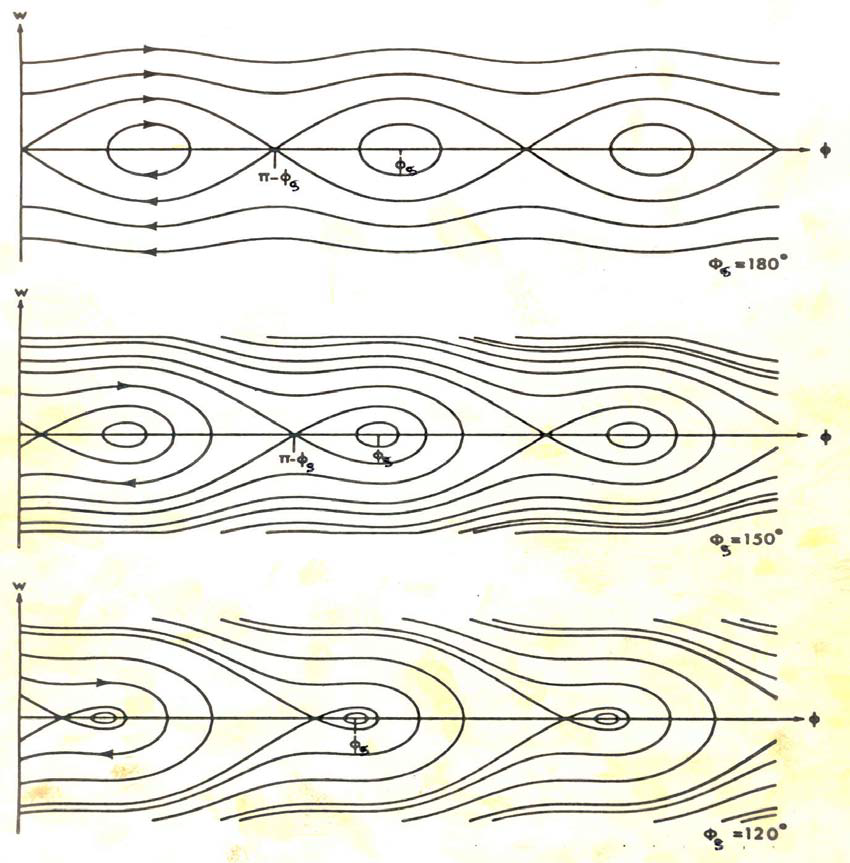
\includegraphics[width=0.75\textwidth]{appendices/figures/longPhaseDiag.png}
\end{center}
\caption{The seperatrix for different synchronous phase values. Note that the acceptance decreases as $\phi_{s} \rightarrow \pi / 2$.}
\label{fig:longSynFreq}
\end{figure}